\begin{table*}[h]

~~~~~~~~~~~~~~~~~~~~~~~~~~~~~~~~~~~~
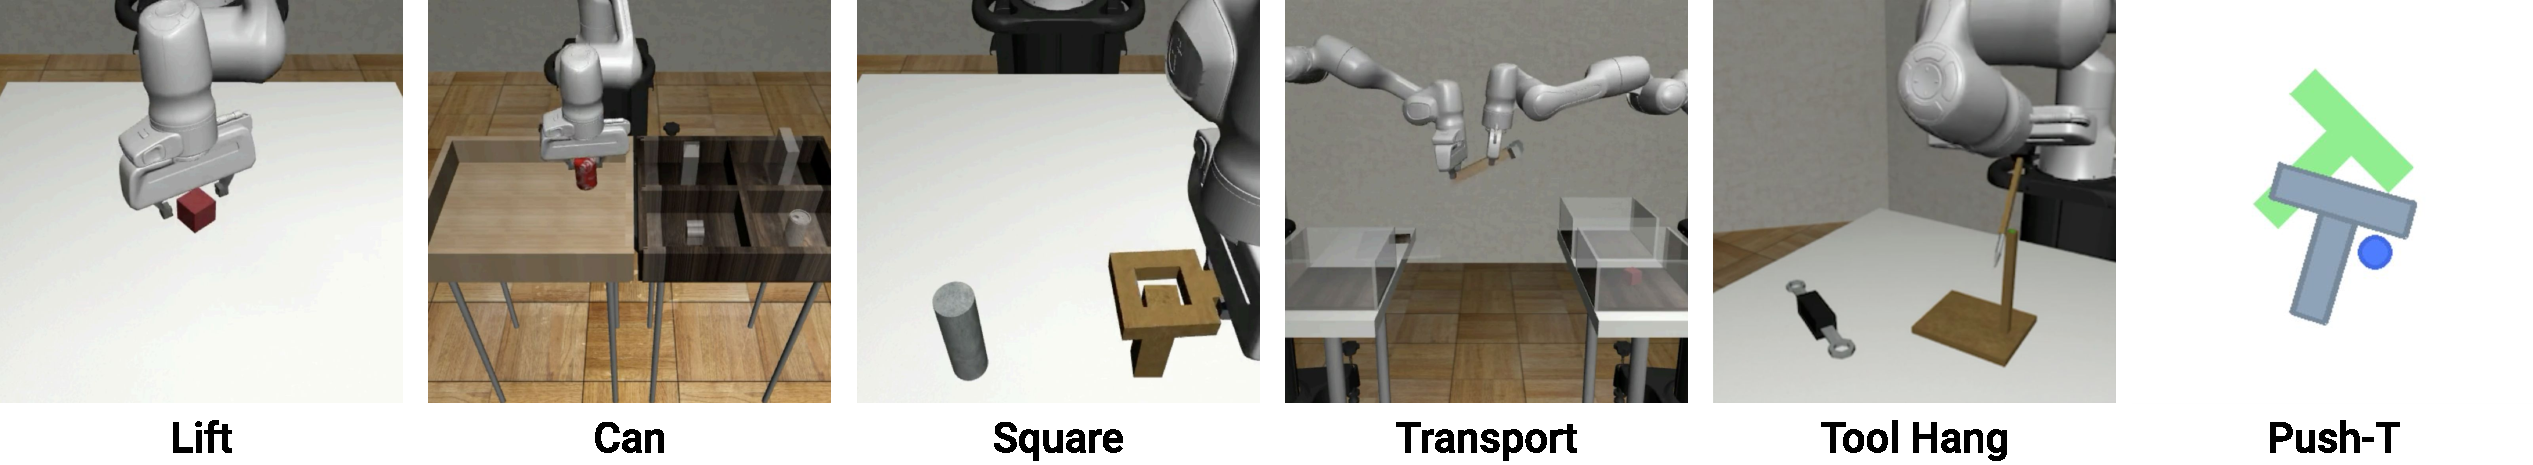
\includegraphics[width=0.835\linewidth]{figure/sim_task_thumbnails.pdf}
\label{tab:sim_benchmark_state}

\vspace{1mm}
{
\centering
% \setlength\tabcolsep{ 4.4 pt}
% \begin{tabular}{r|cc|cc|cc|cc|c|c}
% \toprule

%  & \multicolumn{2}{c|}{ Lift} & \multicolumn{2}{c|}{ Can} & \multicolumn{2}{c|}{ Square} & \multicolumn{2}{c|}{ Transport} & \multicolumn{1}{c|}{ ToolHang} & \multicolumn{1}{c}{ PushT} \\
%  & ph & mh & ph & mh & ph & mh & ph & mh & ph & ph \\
% \midrule
% LSTM-GMM \cite{robomimic} & \small \textbf{1.00}/.960 & \small \textbf{1.00}/.926 & \small \textbf{1.00}/.912 & \small \textbf{1.00}/.806 & \small .955/.732 & \small .864/.588 & \small .758/.467 & \small .621/.199 & \small .667/.312 & \small .896/.832 \\
% IBC  \cite{ibc} & \small .000/.000 & \small .000/.000 & \small .000/.000 & \small .000/.000 & \small .000/.000 & \small .000/.000 & \small .000/.000 & \small .000/.000 & \small .000/.000 & \small .000/.000 \\
% BET & \small \textbf{1.00}/.961 & \small \textbf{1.00}/.992 & \small \textbf{1.00}/.892 & \small \textbf{1.00}/.897 & \small .758/.520 & \small .682/.427 & \small .379/.145 & \small .212/.064 & \small .576/.200 & \small .797/.713 \\
% \midrule
% DiffusionPolicy-C & \small \textbf{1.00}/.985 & \small \textbf{1.00}/.970 & \small \textbf{1.00}/.959 & \small \textbf{1.00}/\textbf{.961} & \small \textbf{1.00}/\textbf{.929} & \small \textbf{.970}/\textbf{.821} & \small .939/.821 & \small \textbf{.682}/\textbf{.455} & \small .515/.221 & \small .994/\textbf{.992} \\
% DiffusionPolicy-T & \small \textbf{1.00}/\textbf{1.00} & \small \textbf{1.00}/\textbf{.999} & \small \textbf{1.00}/\textbf{.996} & \small \textbf{1.00}/.939 & \small \textbf{1.00}/.886 & \small .955/.812 & \small \textbf{1.00}/\textbf{.841} & \small .622/.351 & \small \textbf{1.00}/\textbf{.873} & \small \textbf{1.00}/.991 \\
% \bottomrule
% \end{tabular}

% this version uses number from the original paper (Robomimic)
% \setlength\tabcolsep{ 4.4 pt}
% \begin{tabular}{r|cc|cc|cc|cc|c|c}
% \toprule
%  & \multicolumn{2}{c|}{Lift} & \multicolumn{2}{c|}{Can} & \multicolumn{2}{c|}{Square} & \multicolumn{2}{c|}{Transport} & \multicolumn{1}{c|}{ToolHang} & \multicolumn{1}{c}{PushT} \\
%  & ph & mh & ph & mh & ph & mh & ph & mh & ph & ph \\
% \midrule
% LSTM-GMM \cite{robomimic} & \small \textbf{1.00}/0.96 & \small \textbf{1.00}/0.93 & \small \textbf{1.00}/0.91 & \small \textbf{1.00}/0.81 & \small 0.84/0.73 & \small 0.78/0.59 & \small 0.71/0.47 & \small 0.65/0.20 & \small 0.19/0.31 & \small 0.67/0.61 \\
% IBC \cite{ibc} & \small 0.79/0.41 & \small 0.15/0.02 & \small 0.00/0.00 & \small 0.01/0.01 & \small 0.00/0.00 & \small 0.00/0.00 & \small 0.00/0.00 & \small 0.00/0.00 & \small 0.00/0.00 & \small 0.90/0.84 \\
% BET \cite{bet} & \small \textbf{1.00}/0.96 & \small \textbf{1.00}/0.99 & \small \textbf{1.00}/0.89 & \small \textbf{1.00}/0.90 & \small 0.76/0.52 & \small 0.68/0.43 & \small 0.38/0.14 & \small 0.21/0.06 & \small 0.58/0.20 & \small 0.79/0.70 \\
% \midrule
% DiffusionPolicy-C & \small \textbf{1.00}/0.98 & \small \textbf{1.00}/0.97 & \small \textbf{1.00}/0.96 & \small \textbf{1.00}/\textbf{0.96} & \small \textbf{1.00}/\textbf{0.93} & \small \textbf{0.97}/\textbf{0.82} & \small 0.94/0.82 & \small \textbf{0.68}/\textbf{0.46} & \small 0.50/0.30 & \small 0.95/\textbf{0.91} \\
% DiffusionPolicy-T & \small \textbf{1.00}/\textbf{1.00} & \small \textbf{1.00}/\textbf{1.00} & \small \textbf{1.00}/\textbf{1.00} & \small \textbf{1.00}/0.94 & \small \textbf{1.00}/0.89 & \small 0.95/0.81 & \small \textbf{1.00}/\textbf{0.84} & \small 0.62/0.35 & \small \textbf{1.00}/\textbf{0.87} & \small \textbf{0.95}/0.79 \\
% \bottomrule
% \end{tabular}


% this version uses number we ran
\setlength\tabcolsep{ 3 pt}
\begin{tabular}{r|cc|cc|cc|cc|c|c}
\toprule
 & \multicolumn{2}{c|}{Lift} & \multicolumn{2}{c|}{Can} & \multicolumn{2}{c|}{Square} & \multicolumn{2}{c|}{Transport} & \multicolumn{1}{c|}{ToolHang} & \multicolumn{1}{c}{Push-T} \\
 & ph & mh & ph & mh & ph & mh & ph & mh & ph & ph \\
\midrule
LSTM-GMM & \small \textbf{1.00}/0.96 & \small \textbf{1.00}/0.93 & \small \textbf{1.00}/0.91 & \small \textbf{1.00}/0.81 & \small 0.95/0.73 & \small 0.86/0.59 & \small 0.76/0.47 & \small 0.62/0.20 & \small 0.67/0.31 & \small 0.67/0.61 \\
IBC & \small 0.79/0.41 & \small 0.15/0.02 & \small 0.00/0.00 & \small 0.01/0.01 & \small 0.00/0.00 & \small 0.00/0.00 & \small 0.00/0.00 & \small 0.00/0.00 & \small 0.00/0.00 & \small 0.90/0.84 \\
BET & \small \textbf{1.00}/0.96 & \small \textbf{1.00}/0.99 & \small \textbf{1.00}/0.89 & \small \textbf{1.00}/0.90 & \small 0.76/0.52 & \small 0.68/0.43 & \small 0.38/0.14 & \small 0.21/0.06 & \small 0.58/0.20 & \small 0.79/0.70 \\
\midrule
DiffusionPolicy-C & \small \textbf{1.00}/0.98 & \small \textbf{1.00}/0.97 & \small \textbf{1.00}/0.96 & \small \textbf{1.00}/\textbf{0.96} & \small \textbf{1.00}/\textbf{0.93} & \small \textbf{0.97}/\textbf{0.82} & \small 0.94/0.82 & \small \textbf{0.68}/\textbf{0.46} & \small 0.50/0.30 & \small 0.95/\textbf{0.91} \\
DiffusionPolicy-T & \small \textbf{1.00}/\textbf{1.00} & \small \textbf{1.00}/\textbf{1.00} & \small \textbf{1.00}/\textbf{1.00} & \small \textbf{1.00}/0.94 & \small \textbf{1.00}/0.89 & \small 0.95/0.81 & \small \textbf{1.00}/\textbf{0.84} & \small 0.62/0.35 & \small \textbf{1.00}/\textbf{0.87} & \small \textbf{0.95}/0.79 \\
\bottomrule
\end{tabular}

% Feb 28 update, reran diffusion cnn with obs global cond
% \setlength\tabcolsep{ 4.4 pt}
% \begin{tabular}{r|cc|cc|cc|cc|c|c}
% \toprule
%  & \multicolumn{2}{c|}{Lift} & \multicolumn{2}{c|}{Can} & \multicolumn{2}{c|}{Square} & \multicolumn{2}{c|}{Transport} & \multicolumn{1}{c|}{ToolHang} & \multicolumn{1}{c}{PushT} \\
%  & ph & mh & ph & mh & ph & mh & ph & mh & ph & ph \\
% \midrule
% LSTM-GMM \cite{robomimic} & \small \textbf{1.00}/0.96 & \small \textbf{1.00}/0.93 & \small \textbf{1.00}/0.91 & \small \textbf{1.00}/0.81 & \small 0.84/0.73 & \small 0.78/0.59 & \small 0.71/0.47 & \small 0.65/0.20 & \small 0.19/0.31 & \small 0.67/0.61 \\
% IBC \cite{ibc} & \small 0.79/0.41 & \small 0.15/0.02 & \small 0.00/0.00 & \small 0.01/0.01 & \small 0.00/0.00 & \small 0.00/0.00 & \small 0.00/0.00 & \small 0.00/0.00 & \small 0.00/0.00 & \small 0.90/0.84 \\
% BET & \small \textbf{1.00}/0.96 & \small \textbf{1.00}/0.99 & \small \textbf{1.00}/0.89 & \small \textbf{1.00}/0.90 & \small 0.76/0.52 & \small 0.68/0.43 & \small 0.38/0.14 & \small 0.21/0.06 & \small 0.58/0.20 & \small 0.79/0.70 \\
% DiffusionPolicy-C & \small \textbf{1.00}/\textbf{1.00} & \small \textbf{1.00}/0.98 & \small \textbf{1.00}/\textbf{1.00} & \small \textbf{1.00}/\textbf{0.99} & \small \textbf{1.00}/\textbf{0.95} & \small \textbf{0.98}/\textbf{0.86} & \small 0.95/\textbf{0.85} & \small \textbf{0.77}/\textbf{0.60} & \small 0.86/0.52 & \small 0.95/\textbf{0.91} \\
% DiffusionPolicy-T & \small \textbf{1.00}/\textbf{1.00} & \small \textbf{1.00}/\textbf{1.00} & \small \textbf{1.00}/1.00 & \small \textbf{1.00}/0.94 & \small \textbf{1.00}/0.89 & \small 0.95/0.81 & \small \textbf{1.00}/0.84 & \small 0.62/0.35 & \small \textbf{1.00}/\textbf{0.87} & \small \textbf{0.95}/0.79 \\
% \bottomrule
% \end{tabular}


\caption{\textbf{Behavior Cloning Benchmark (State Policy) \label{tab:table_low_dim} }
We present success rates with different checkpoint selection methods in the format of (max performance) / (average of last 10 checkpoints), with each averaged across 3 training seeds and 50 different environment initial conditions (150 in total).
LSTM-GMM corresponds to BC-RNN in RoboMimic\cite{robomimic}, which we reproduced and obtained slightly {better} results than the original paper. Our results show that Diffusion Policy significantly improves state-of-the-art performance across the board.
}
\vspace{2mm}


% \setlength\tabcolsep{ 4.4 pt}
% \begin{tabular}{r|cc|cc|cc|cc|c|c}
% \toprule
%  & \multicolumn{2}{c|}{ Lift} & \multicolumn{2}{c|}{ Can} & \multicolumn{2}{c|}{ Square} & \multicolumn{2}{c|}{ Transport} & \multicolumn{1}{c|}{ ToolHang} & \multicolumn{1}{c}{ PushT} \\
%  & ph & mh & ph & mh & ph & mh & ph & mh & ph & ph \\
% \midrule
% LSTM-GMM \cite{robomimic} & \small \textbf{1.00}/.000 & \small \textbf{1.00}/.000 & \small .980/.000 & \small .960/.000 & \small .820/.000 & \small .767/.000 & \small .720/.000 & \small .420/.000 & \small .673/.000 & \small .782/.690 \\
% IBC \cite{ibc} & \small .000/.000 & \small .000/.000 & \small .000/.000 & \small .000/.000 & \small .000/.000 & \small .000/.000 & \small .000/.000 & \small .000/.000 & \small .000/.000 & \small .000/.000 \\

% \midrule
% DiffusionPolicy-C & \small \textbf{1.00}/\textbf{1.00} & \small \textbf{1.00}/\textbf{.997} & \small \textbf{1.00}/.974 & \small \textbf{1.00}/\textbf{.962} & \small .985/\textbf{.923} & \small .924/.674 & \small \textbf{.955}/.712 & \small \textbf{.697}/\textbf{.489} & \small \textbf{.849}/\textbf{.614} & \small \textbf{.984}/\textbf{.937} \\
% DiffusionPolicy-T & \small \textbf{1.00}/\textbf{1.00} & \small \textbf{1.00}/.992 & \small \textbf{1.00}/\textbf{.979} & \small \textbf{1.00}/.958 & \small \textbf{1.00}/.900 & \small \textbf{.939}/\textbf{.841} & \small .839/\textbf{.762} & \small .530/.346 & \small .712/.472 & \small .909/.810 \\
% \bottomrule
% \end{tabular}

% this version uses number from the paper
% \setlength\tabcolsep{ 4.4 pt}
% \begin{tabular}{r|cc|cc|cc|cc|c|c}
% \toprule
%  & \multicolumn{2}{c|}{Lift} & \multicolumn{2}{c|}{Can} & \multicolumn{2}{c|}{Square} & \multicolumn{2}{c|}{Transport} & \multicolumn{1}{c|}{ToolHang} & \multicolumn{1}{c}{PushT} \\
%  & ph & mh & ph & mh & ph & mh & ph & mh & ph & ph \\
% \midrule
% LSTM-GMM \cite{robomimic} & \small \textbf{1.00}/0.96 & \small \textbf{1.00}/0.95 & \small 0.98/0.88 & \small 0.96/0.90 & \small 0.82/0.59 & \small 0.77/0.38 & \small 0.72/0.62 & \small 0.42/0.23 & \small 0.67/0.49 & \small 0.69/0.54 \\
% IBC \cite{ibc} & \small 0.94/0.73 & \small 0.39/0.05 & \small 0.08/0.01 & \small 0.00/0.00 & \small 0.03/0.00 & \small 0.00/0.00 & \small 0.00/0.00 & \small 0.00/0.00 & \small 0.00/0.00 & \small 0.75/0.64 \\
% \midrule
% DiffusionPolicy-C & \small \textbf{1.00}/\textbf{1.00} & \small \textbf{1.00}/\textbf{1.00} & \small \textbf{1.00}/0.97 & \small \textbf{1.00}/0.96 & \small 0.98/\textbf{0.92} & \small \textbf{0.98}/\textbf{0.84} & \small \textbf{1.00}/\textbf{0.93} & \small \textbf{0.86}/\textbf{0.71} & \small \textbf{0.95}/\textbf{0.79} & \small \textbf{0.91}/\textbf{0.84} \\
% DiffusionPolicy-T & \small \textbf{1.00}/\textbf{1.00} & \small \textbf{1.00}/0.99 & \small \textbf{1.00}/\textbf{0.98} & \small \textbf{1.00}/\textbf{0.98} & \small \textbf{1.00}/0.90 & \small 0.94/0.80 & \small 0.98/0.81 & \small 0.71/0.48 & \small 0.76/0.47 & \small 0.78/0.66 \\
% \bottomrule
% \end{tabular}

% this version uses number from our experiments
% \setlength\tabcolsep{ 4.4 pt}
% \begin{tabular}{r|cc|cc|cc|cc|c|c}
% \toprule
%  & \multicolumn{2}{c|}{Lift} & \multicolumn{2}{c|}{Can} & \multicolumn{2}{c|}{Square} & \multicolumn{2}{c|}{Transport} & \multicolumn{1}{c|}{ToolHang} & \multicolumn{1}{c}{PushT} \\
%  & ph & mh & ph & mh & ph & mh & ph & mh & ph & ph \\
% \midrule
% LSTM-GMM \cite{robomimic} & \small \textbf{1.00}/0.96 & \small \textbf{1.00}/0.95 & \small 0.98/0.88 & \small 0.96/0.90 & \small 0.82/0.59 & \small 0.77/0.38 & \small 0.72/0.62 & \small 0.42/0.24 & \small 0.67/0.49 & \small 0.69/0.54 \\
% IBC \cite{ibc} & \small 0.94/0.73 & \small 0.39/0.05 & \small 0.08/0.01 & \small 0.00/0.00 & \small 0.03/0.00 & \small 0.00/0.00 & \small 0.00/0.00 & \small 0.00/0.00 & \small 0.00/0.00 & \small 0.75/0.64 \\
% DiffusionPolicy-C & \small \textbf{1.00}/\textbf{1.00} & \small \textbf{1.00}/\textbf{1.00} & \small \textbf{1.00}/0.97 & \small \textbf{1.00}/0.96 & \small 0.98/\textbf{0.92} & \small \textbf{0.98}/\textbf{0.84} & \small \textbf{1.00}/\textbf{0.93} & \small \textbf{0.89}/\textbf{0.69} & \small \textbf{0.95}/\textbf{0.73} & \small \textbf{0.91}/\textbf{0.84} \\
% DiffusionPolicy-T & \small \textbf{1.00}/\textbf{1.00} & \small \textbf{1.00}/0.99 & \small \textbf{1.00}/\textbf{0.98} & \small \textbf{1.00}/\textbf{0.98} & \small \textbf{1.00}/0.90 & \small 0.94/0.80 & \small 0.98/0.81 & \small 0.73/0.50 & \small 0.76/0.47 & \small 0.78/0.66 \\
% \bottomrule
% \end{tabular}

\setlength\tabcolsep{ 3 pt}
\begin{tabular}{r|cc|cc|cc|cc|c|c}
\toprule
 & \multicolumn{2}{c|}{Lift} & \multicolumn{2}{c|}{Can} & \multicolumn{2}{c|}{Square} & \multicolumn{2}{c|}{Transport} & \multicolumn{1}{c|}{ToolHang} & \multicolumn{1}{c}{Push-T} \\
 & ph & mh & ph & mh & ph & mh & ph & mh & ph & ph \\
\midrule
LSTM-GMM & \small \textbf{1.00}/0.96 & \small \textbf{1.00}/0.95 & \small \textbf{1.00}/0.88 & \small 0.98/0.90 & \small 0.82/0.59 & \small 0.64/0.38 & \small 0.88/0.62 & \small 0.44/0.24 & \small 0.68/0.49 & \small 0.69/0.54 \\
IBC & \small 0.94/0.73 & \small 0.39/0.05 & \small 0.08/0.01 & \small 0.00/0.00 & \small 0.03/0.00 & \small 0.00/0.00 & \small 0.00/0.00 & \small 0.00/0.00 & \small 0.00/0.00 & \small 0.75/0.64 \\
DiffusionPolicy-C & \small \textbf{1.00}/\textbf{1.00} & \small \textbf{1.00}/\textbf{1.00} & \small \textbf{1.00}/0.97 & \small \textbf{1.00}/0.96 & \small 0.98/\textbf{0.92} & \small \textbf{0.98}/\textbf{0.84} & \small \textbf{1.00}/\textbf{0.93} & \small \textbf{0.89}/\textbf{0.69} & \small \textbf{0.95}/\textbf{0.73} & \small \textbf{0.91}/\textbf{0.84} \\
DiffusionPolicy-T & \small \textbf{1.00}/\textbf{1.00} & \small \textbf{1.00}/0.99 & \small \textbf{1.00}/\textbf{0.98} & \small \textbf{1.00}/\textbf{0.98} & \small \textbf{1.00}/0.90 & \small 0.94/0.80 & \small 0.98/0.81 & \small 0.73/0.50 & \small 0.76/0.47 & \small 0.78/0.66 \\
\bottomrule
\end{tabular}

\caption{\textbf{Behavior Cloning Benchmark (Visual Policy) \label{tab:table_image}} Performance are reported in the same format as in Tab \ref{tab:table_low_dim}. LSTM-GMM numbers were reproduced to get a complete evaluation in addition to the best checkpoint performance reported. Diffusion Policy shows consistent performance improvement, especially for complex tasks like Transport and ToolHang. }
}
\end{table*}

\section{Evaluation}
We systematically evaluate Diffusion Policy on 15 tasks from 4 benchmarks \cite{ibc, gupta2019relay, robomimic, bet}. This evaluation suite includes both simulated and real environments, single and multiple task benchmarks, fully actuated and under-actuated systems, and rigid and fluid objects.  We found Diffusion Policy to consistently outperform the prior state-of-the-art on all of the tested benchmarks, with an average success-rate improvement of 46.9\%. In the following sections, we  provide an overview of each task, our evaluation methodology on that task, and our key takeaways.

\subsection{Simulation Environments and datasets}
\textbf{Robomimic}
\cite{robomimic} is a large-scale robotic manipulation benchmark designed to study imitation learning and offline RL. The benchmark consists of 5 tasks with a proficient human (PH) teleoperated demonstration dataset for each and mixed proficient/non-proficient human (MH) demonstration datasets for 4 of the tasks (9 variants in total). For each variant, we report results for both state- and image-based observations. Properties for each task are summarized in Tab \ref{tab:robomimic_tasks}.

\begin{table}
\centering
\setlength\tabcolsep{2 pt}
\small
\begin{tabular}{c|cccccccc}
\toprule
Task      & \# Rob & \# Obj & ActD & \#PH & \#MH & Steps & Img? & HiPrec \\
\midrule
\multicolumn{1}{c}{} & \multicolumn{8}{c}{Simulation Benchmark} \\
\midrule
Lift      & 1      & 1      & 7    & 200   & 300   & 400       & Yes    & No       \\
Can       & 1      & 1      & 7    & 200   & 300   & 400       & Yes    & No       \\
Square    & 1      & 1      & 7    & 200   & 300   & 400       & Yes    & Yes      \\
Transport & 2      & 3      & 14   & 200   & 300   & 700       & Yes    & No       \\
ToolHang  & 1      & 2      & 7    & 200   & 0     & 700       & Yes    & Yes      \\
\midrule
Push-T    & 1      & 1      & 2    & 200   & 0     & 300       & Yes    & Yes      \\
\midrule
BlockPush & 1      & 2      & 2    & 0     & 0     & 350       & No     & No       \\
\midrule
Kitchen   & 1      & 7      & 9    & 656   & 0     & 280       & No     & No      \\
\midrule
\multicolumn{1}{c}{} & \multicolumn{8}{c}{Realworld Benchmark} \\
\midrule
Push-T    & 1      & 1      & 2    & 136   & 0     & 600       & Yes    & Yes  \\
6DoF Pour   & 1    & liquid      & 6    & 90   & 0     & 600       & Yes    & No  \\
Peri Spread   & 1      & liquid      & 6    & 90   & 0     & 600       & Yes    & No  \\
Mug Flip  & 1      & 1      & 7    & 250   & 0     & 600       & Yes    & No  \\
\bottomrule
\end{tabular}

\caption{\textbf{Tasks Summary.} \# Rob: number of robots, \#Obj: number of objects, ActD: action dimension, PH: proficient-human demonstration, MH: multi-human demonstration, Steps: max number of rollout steps, HiPrec: whether the task has a high precision requirement. BlockPush uses 1000 episodes of scripted  demonstrations.}
\label{tab:robomimic_tasks}
\vspace{-5mm}
\end{table}

\textbf{Push-T}
\label{sec:eval_sim_pusht}
adapted from IBC \cite{ibc}, requires pushing a T-shaped block (gray) to a fixed target (red) with a circular end-effector (blue)s. Variation is added by random initial conditions for T block and end-effector. The task requires exploiting complex and contact-rich object dynamics to push the T block precisely, using point contacts. There are two variants: one with RGB image observations and another with 9 2D keypoints obtained from the ground-truth pose of the T block, both with proprioception for end-effector location.

\textbf{Multimodal Block Pushing} adapted from BET \cite{bet}, this task tests the policy's ability to model multimodal action distributions by pushing two blocks into two squares in any order. The demonstration data is generated by a scripted oracle with access to groundtruth state info. This oracle randomly selects an initial block to push and moves it to a randomly selected square. The remaining block is then pushed into the remaining square. This task contains \textbf{long-horizon} multimodality that can not be modeled by a single function mapping from observation to action.

\textbf{Franka Kitchen} is a popular environment for evaluating the ability of IL and Offline-RL methods to learn multiple long-horizon tasks. Proposed in Relay Policy Learning \cite{gupta2019relay}, the Franka Kitchen environment contains 7 objects for interaction and comes with a human demonstration dataset of 566 demonstrations, each completing 4 tasks in arbitrary order. The goal is to execute as many demonstrated tasks as possible, regardless of order, showcasing both short-horizon and long-horizon multimodality.

\begin{table}[t]
\centering
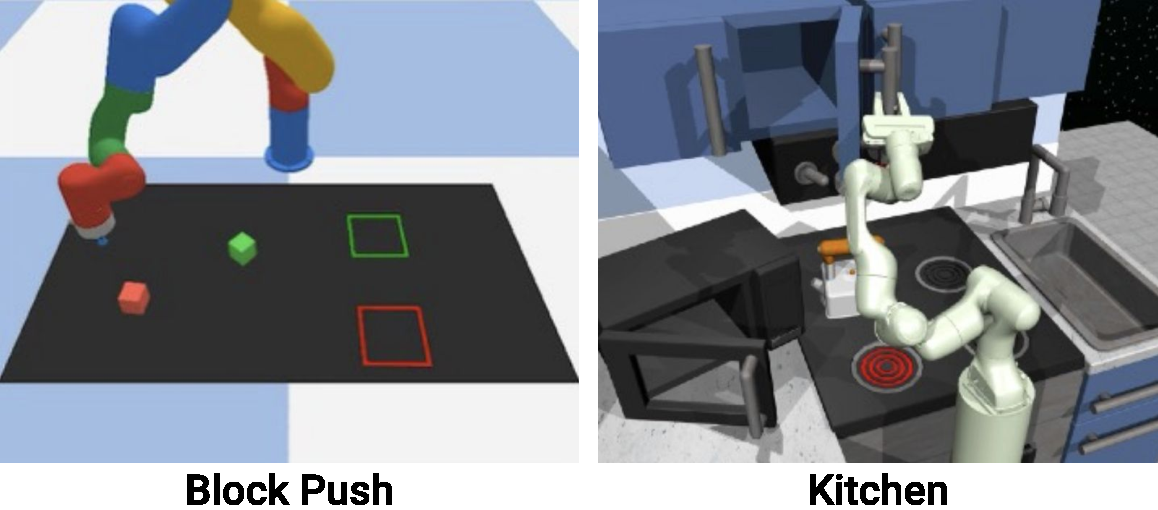
\includegraphics[width=0.9\linewidth]{figure/multitask_thumbnails.pdf}

\vspace{2mm}



\setlength\tabcolsep{4.8 pt}
\begin{tabular}{r|cc|cccc}
\toprule
 & \multicolumn{2}{c|}{BlockPush} & \multicolumn{4}{c}{Kitchen} \\
 & p1 & p2 & p1 & p2 & p3 & p4 \\
\midrule
LSTM-GMM & \small 0.03 & \small 0.01 & \small \textbf{1.00} & \small 0.90 & \small 0.74 & \small 0.34 \\
IBC & \small 0.01 & \small 0.00 & \small 0.99 & \small 0.87 & \small 0.61 & \small 0.24 \\
BET & \small 0.96 & \small 0.71 & \small 0.99 & \small 0.93 & \small 0.71 & \small 0.44 \\
DiffusionPolicy-C & \small 0.36 & \small 0.11 & \small \textbf{1.00} & \small \textbf{1.00} & \small \textbf{1.00} & \small \textbf{0.99} \\
DiffusionPolicy-T & \small \textbf{0.99} & \small \textbf{0.94} & \small \textbf{1.00} & \small 0.99 & \small 0.99 & \small 0.96 \\
\bottomrule
\end{tabular}

\caption{\textbf{Multi-Stage Tasks (State Observation)}.
\label{tab:multi_stage}
For PushBlock, $px$ is the frequency of pushing $x$ blocks into the targets.
For Kitchen, $px$ is the frequency of interacting with $x$ or more objects (e.g. bottom burner).
Diffusion Policy performs better, especially for difficult metrics such as $p2$ for Block Pushing and $p4$ for Kitchen, as demonstrated by our results.
}
\vspace{-4mm}
\end{table}

\subsection{Evaluation Methodology}
We present the \textbf{best-performing for each baseline method} on each benchmark from all possible sources -- our reproduced result (LSTM-GMM) or original number reported in the paper (BET, IBC). We report results from the average of the last 10 checkpoints (saved every 50 epochs) across \textbf{3} training seeds and \textbf{50} environment initializations
\footnote{Due to a bug in our evaluation code, only 22 environment initializations are used for robomimic tasks. This does not change our conclusion since all baseline methods are evaluated in the same way.}
(an average of \textbf{1500} experiments in total). The metric for most tasks is success rate, except for the Push-T task, which uses target area coverage.
In addition, we report the average of best-performing checkpoints for robomimic and Push-T tasks to be consistent with the evaluation methodology of their respective original papers \cite{robomimic, ibc}. All state-based tasks are trained for 4500 epochs, and image-based tasks for 3000 epochs. Each method is evaluated with its best-performing action space: position control for Diffusion Policy and velocity control for baselines (the effect of action space will be discussed in detail in Sec \ref{sec:eval_pos_vs_vel}).
The results from these simulation benchmarks are summarized in Table \ref{tab:table_low_dim} and Table \ref{tab:table_image}.


\subsection{Key Findings}

Diffusion Policy outperforms alternative methods on all tasks and variants, with both state and vision observations, in our simulation benchmark study (Tabs \ref{tab:table_low_dim}, \ref{tab:table_image} and \ref{tab:multi_stage}) with an average improvement of 46.9\%. The following paragraphs summarize the key takeaways.


\textbf{Diffusion Policy can express short-horizon multimodality.}
We define short-horizon action multimodality as multiple ways of achieving \textbf{the same immediate goal}, which is prevalent in human demonstration data \cite{robomimic}. %
In Fig \ref{fig:multimodal}, we present a case study of this type of short-horizon multimodality in the Push-T task. Diffusion Policy learns to approach the contact point equally likely from left or right, while LSTM-GMM \cite{robomimic} and IBC \cite{ibc} exhibit bias toward one side and BET \cite{bet} cannot commit to one mode.





\textbf{Diffusion Policy can express long-horizon multimodality.}
Long-horizon multimodality is the completion of \textbf{different sub-goals} in inconsistent order. For example, the order of pushing a particular block in the Block Push task or the order of interacting with 7 possible objects in the Kitchen task are arbitrary.
We find that Diffusion Policy copes well with this type of multimodality; it outperforms baselines on both tasks by a large margin: 32\% improvement on Block Push's p2 metric and 213\% improvement on Kitchen's p4 metric.

\textbf{Diffusion Policy can better leverage position control.}
\label{sec:eval_pos_vs_vel}
Our ablation study (Fig. \ref{fig:pos_vs_vel}) shows that selecting position control as the diffusion-policy action space significantly outperformed velocity control. The baseline methods we evaluate, however, work best with velocity control (and this is reflected in the literature where most existing work reports using velocity-control action spaces \cite{robomimic, bet, zhang2018deep, florence2019self, mandlekar2020learning, mandlekar2020iris}).



\textbf{The tradeoff in action horizon.}
As discussed in Sec \ref{sec:action_sequence},
having an action horizon greater than 1 helps the policy predict consistent actions and compensate for idle portions of the demonstration, but too long a horizon reduces performance due to slow reaction time. Our experiment confirms this trade-off (Fig. \ref{fig:ablation} left) and found the action horizon of 8 steps to be optimal for most tasks that we tested.

\textbf{Robustness against latency.}
Diffusion Policy employs receding horizon position control to predict a sequence of actions into the future. This design helps address the latency gap caused by image processing, policy inference, and network delay. Our ablation study with simulated latency showed Diffusion Policy is able to maintain peak performance with latency up to 4 steps (Fig \ref{fig:ablation}). We also find that velocity control is more affected by latency than position control, likely due to compounding error effects.



\textbf{Diffusion Policy is stable to train.}
We found that the optimal hyperparameters for Diffusion Policy are mostly consistent across tasks.  In contrast,  IBC \cite{ibc} is prone to training instability. This property is discussed in Sec \ref{sec:ibc_stability}.



\subsection{Ablation Study}
\label{sec:arch_ablation}
We explore alternative vision encoder design decisions on the simulated robomimic square task.
Specifically, we evaluated 3 different architectures:
ResNet-18, ResNet-34 \cite{resnet}
and ViT-B/16 \cite{dosovitskiy2020image}.
For each architecture, we evaluated 3 different training strategies:
training end-to-end from scratch,
using frozen pre-trained vision encoder,
and finetuning pre-trained vision encoders (with 10x lower learning rate with respect to the policy network).
We use ImageNet-21k \cite{ridnik2021imagenet21k} pretraining for ResNet and CLIP \cite{radford2021learning} pretraining for ViT-B/16.
The quantitative comparison on square task with proficient-human (PH) dataset is shown in Tab. \ref{tab:ablation_vision_encorder}.

We found training ViT from scratch to be challenging (with only 22\% success rate), likely due to the limited amount data.
We also found training with frozen pretrained vision encoder to yield poor performance, which indicates that diffusion policy prefers different vision representation than what is offered in popular pretraining methods.
However, we found finetuning the pretrained vision encoder with a small learning rate (10x smaller vs diffusion policy network) gives the best performance overall. This is especially true for the CLIP-trained ViT-B/16, which reaches 98\% success rate with only 50 epochs of training.
Overall, the best performance across different architectures is not large, despite their significant theoretical capacity gap. We anticipate that their performance gap could be more pronounced on a complex task.

\begin{table}
\centering
\begin{tabular}{r|c|cc}
\toprule
Archicture \& & From & \multicolumn{2}{c}{Pretrained} \\
Prertain Datset& Scatch & frozen & finetuning \\
\midrule
Resnet18 (in21) & 0.94   & 0.58      & 0.92             \\
Resnet34 (in21)& 0.92   & 0.40      & 0.94             \\
ViT-base (clip)& 0.22   & 0.70      & 0.98             \\
\bottomrule
\end{tabular}
\caption{\textbf{Vision Encoder Comparison} All models are trained on the robomimic square (ph) task using CNN-based diffusion policy. Each model is trained for 500 epochs and evaluated every 50 epochs under 50 different environment initial conditions.}
\label{tab:ablation_vision_encorder}
\vspace{-2mm}
\end{table}


\section{Realworld Evaluation}
We evaluated Diffusion Policy in the realworld performance on 4 tasks across 2 hardware setups -- with training data from different demonstrators for each setup. On the realworld Push-T task, we perform ablations examining Diffusion Policy on 2 architecture options and 3 visual encoder options; we also benchmarked against 2 baseline methods with both position-control and velocity-control action spaces. On all tasks, Diffusion Policy variants with both CNN backbones and end-to-end-trained visual encoders yielded the best performance. More details about the task setup and parameters may be found in supplemental materials.

\begin{table}[t]
\centering
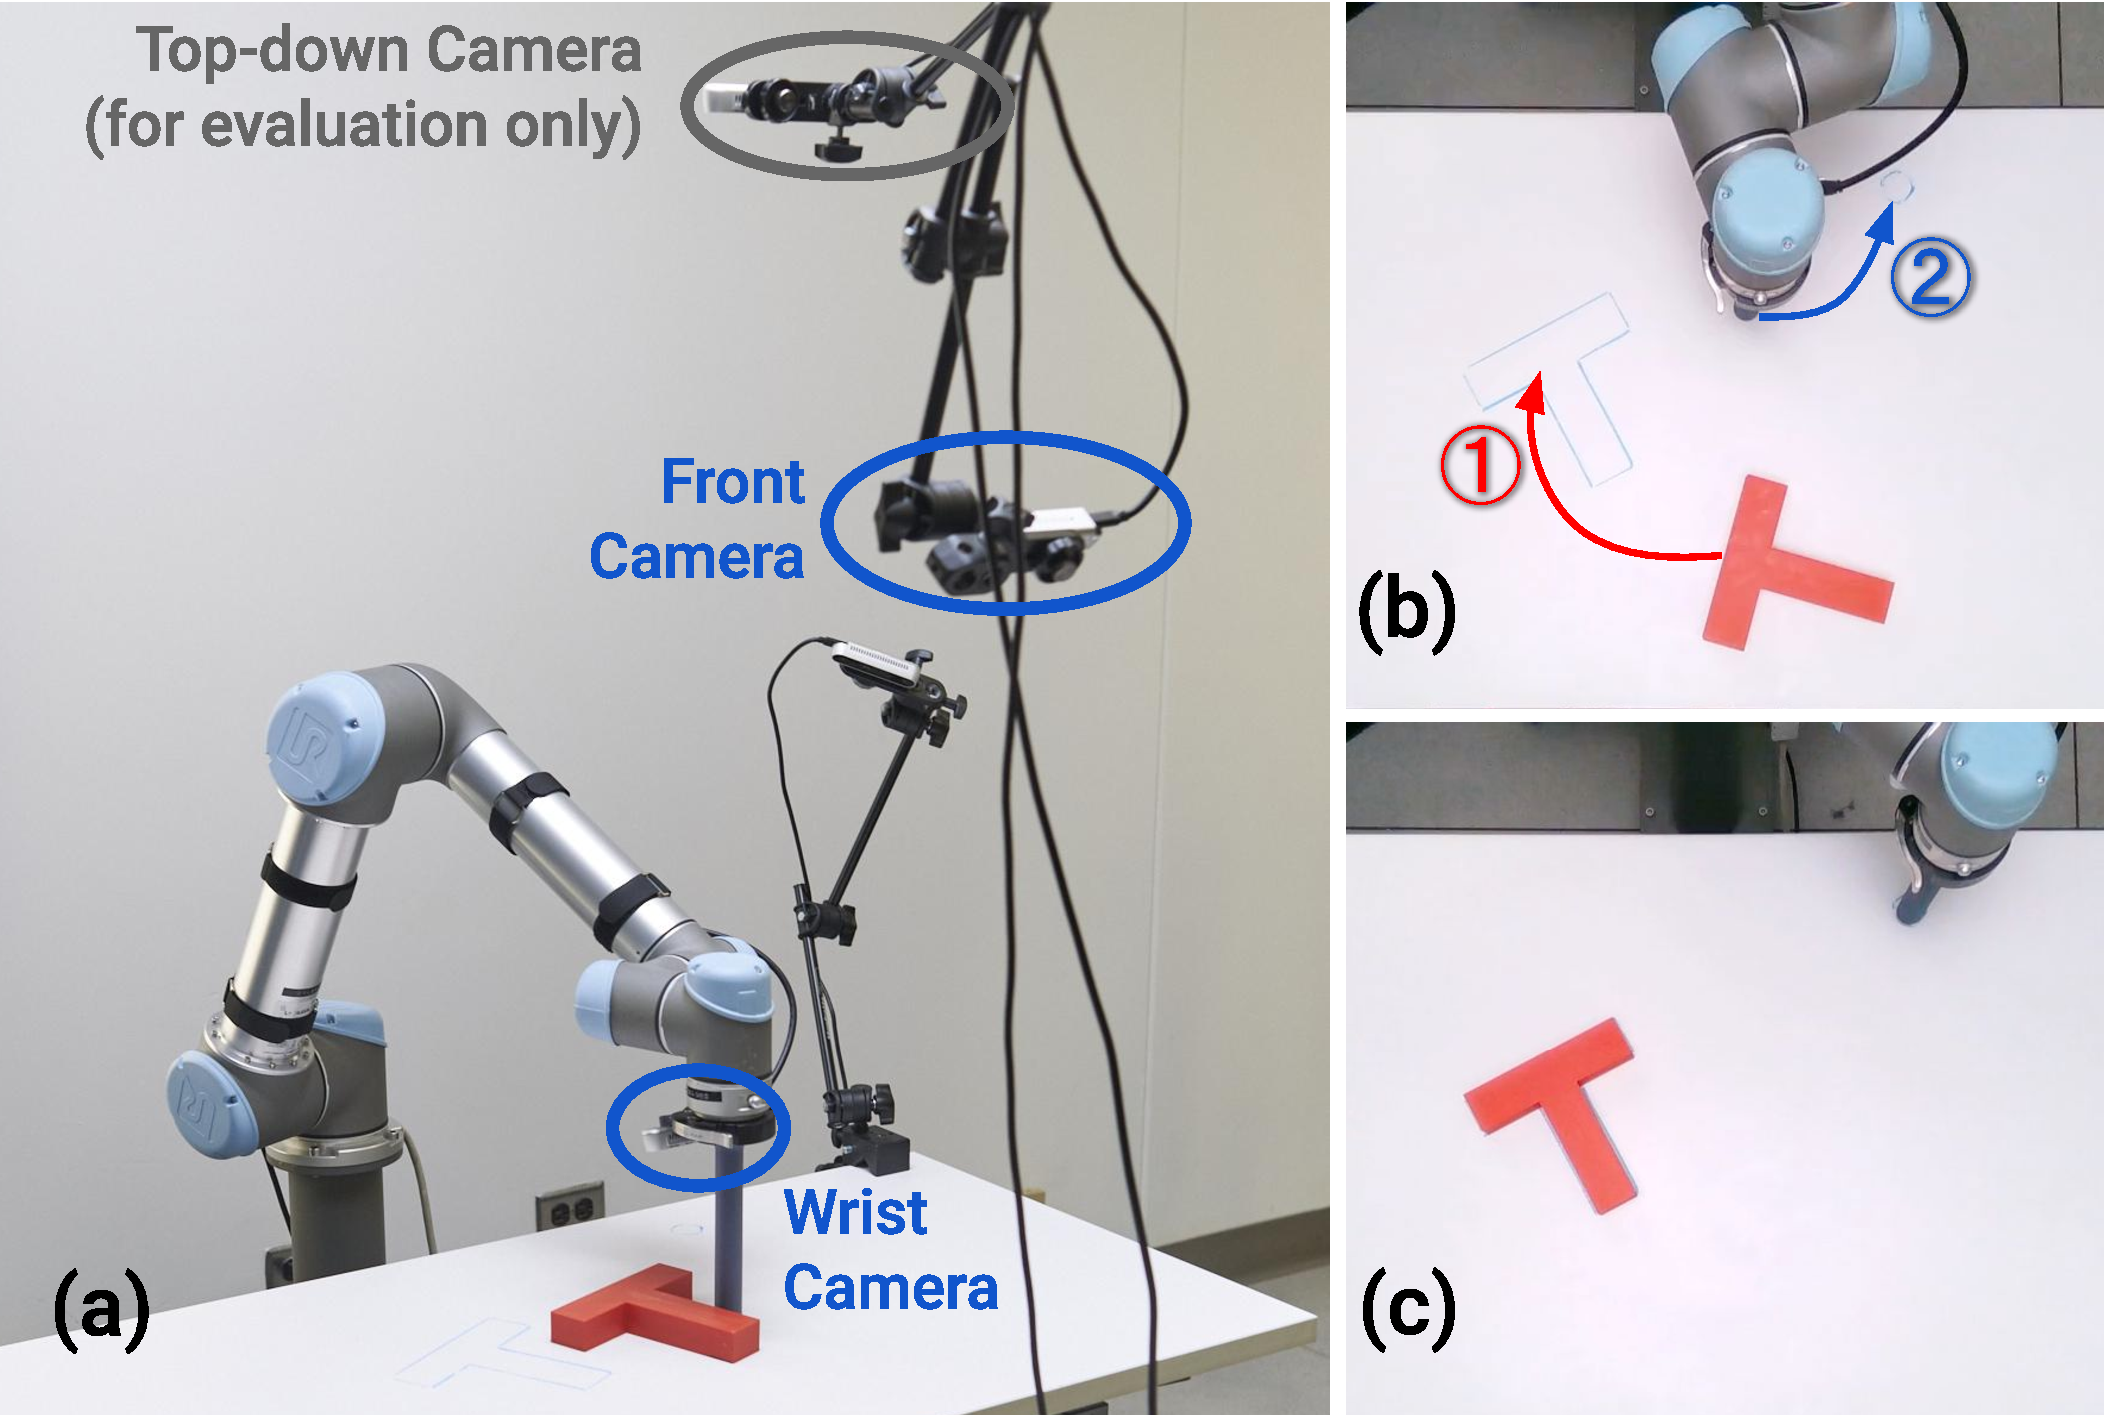
\includegraphics[width=0.9\linewidth]{figure/real_task_setup.pdf}

\vspace{2mm}
\setlength\tabcolsep{1.2pt}
\small
\begin{tabular}{c|c|cc|cc|cccc}
\toprule
       & Human & \multicolumn{2}{c|}{IBC} & \multicolumn{2}{c|}{LSTM-GMM} & \multicolumn{4}{c}{Diffusion Policy}     \\
       & Demo  & pos        & vel        & pos          & vel         & T-E2E & ImgNet & R3M & E2E         \\
\midrule
IoU      & 0.84  & 0.14       & 0.19       & 0.24         & 0.25        & 0.53  & 0.24     & 0.66  & \textbf{0.80} \\
Succ\%   & 1.00  & 0.00       & 0.00       & 0.20         & 0.10        & 0.65  & 0.15     & 0.80  & \textbf{0.95} \\
Dur. & 20.3  & 56.3       & 41.6       & 47.3         & 51.7        & 57.5  & 55.8     & 31.7  & \textbf{22.9} \\
\bottomrule
% https://docs.google.com/spreadsheets/d/1TftzQuEmERMvSM4EpzPl7GZ2mw5Ym024wV2TPW9N6R4/edit#gid=577907863
\end{tabular}


\caption{\textbf{Realworld Push-T Experiment.}
\label{tab:real_pusht}
a) Hardware setup.
b) Illustration of the task. The robot needs to \textcircled{\raisebox{-0.9pt}{1}} precisely push the T-shaped block into the target region, \textbf{and} \textcircled{\raisebox{-0.9pt}{2}} move the end-effector to the end-zone.
c) The ground truth end state used to calculate IoU metrics used in this table. Table: Success is defined by the end-state IoU greater than the minimum IoU in the demonstration dataset. Average episode duration presented in seconds. T-E2E stands for end-to-end trained Transformer-based Diffusion Policy}

\vspace{-4mm}
\end{table}

\begin{figure*}
\centering
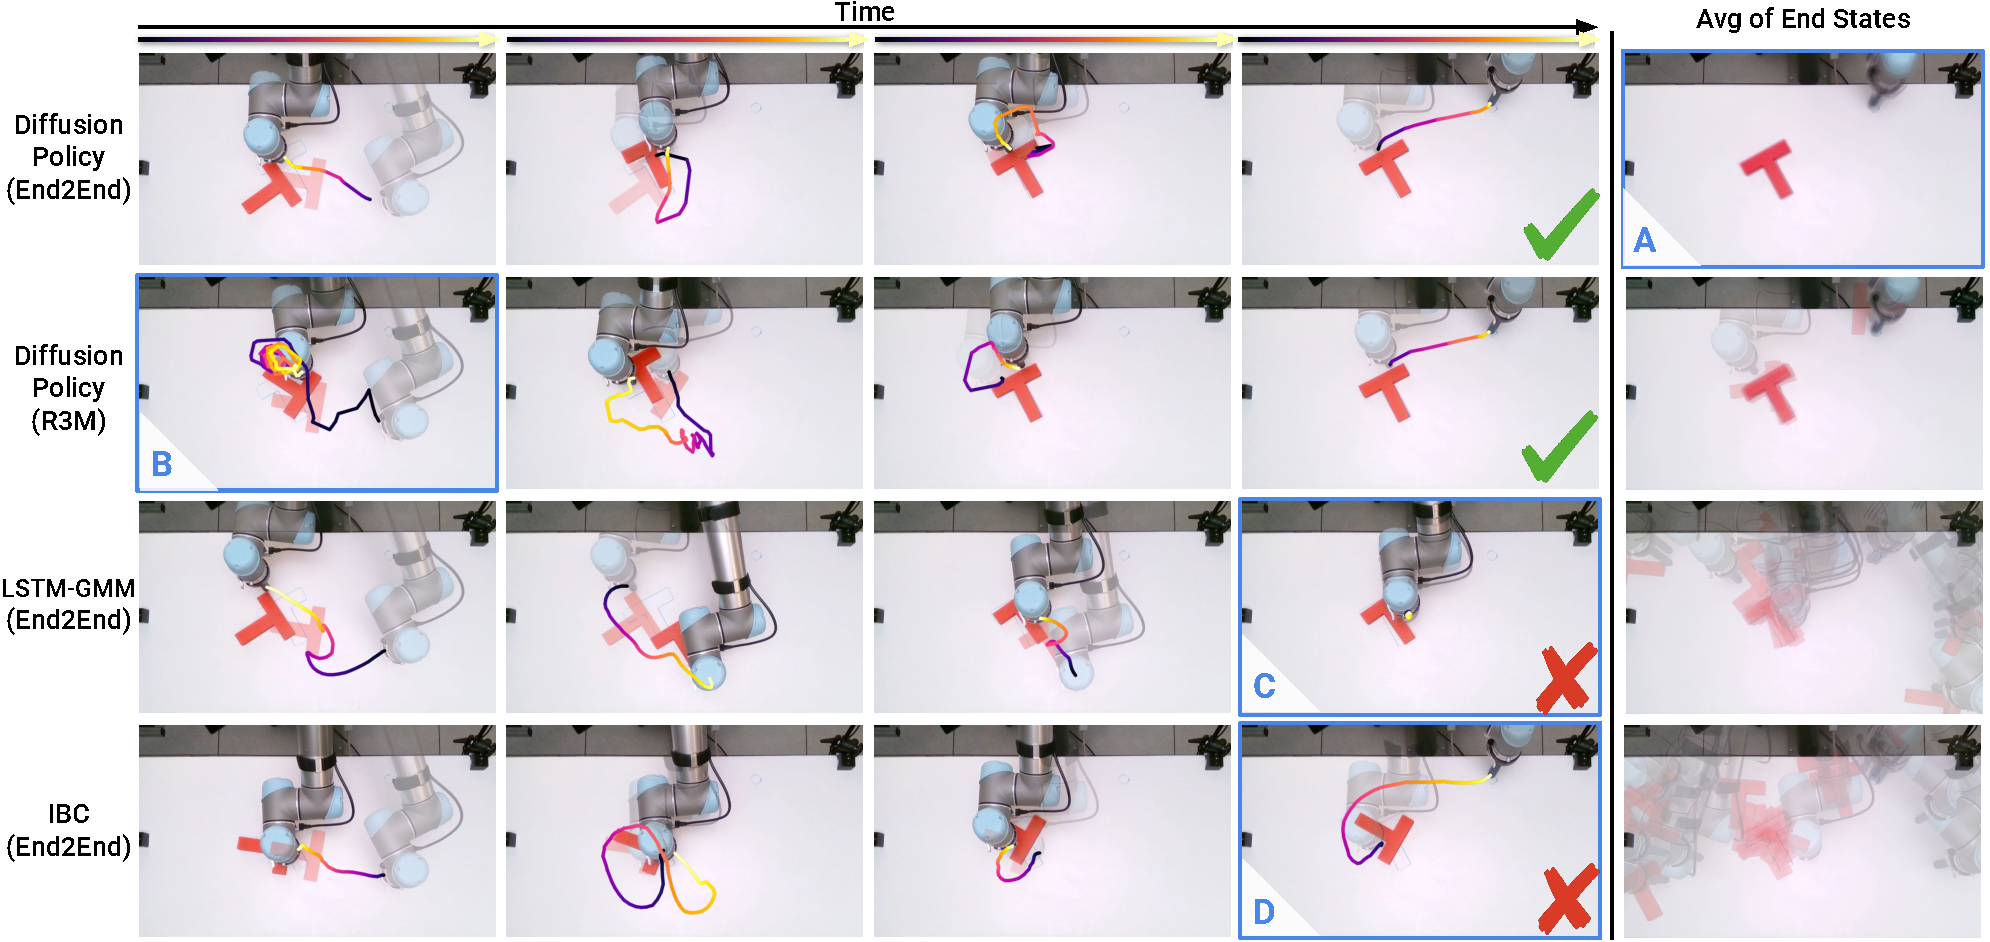
\includegraphics[width=\linewidth]{figure/real_results.pdf}

\caption{\textbf{Realworld Push-T Comparisons.}
\label{fig:real_pusht_comparison}
Columns 1-4 show action trajectories based on key events. The last column shows averaged images of the end state.
\textbf{A}: Diffusion policy (End2End) achieves more accurate and consistent end states.
\textbf{B}: Diffusion Policy (R3M) gets stuck initially but later recovers and finishes the task.
\textbf{C}: LSTM-GMM fails to reach the end zone while adjusting the T block, blocking the eval camera view.
\textbf{D}: IBC prematurely ends the pushing stage.
}
\vspace{-2mm}
\end{figure*}

\subsection{Realworld Push-T Task}

Real-world Push-T is significantly harder than the simulated version due to 3 modifications: 1. The real-world Push-T task is \textbf{multi-stage}. It requires the robot to \textcircled{\raisebox{-0.9pt}{1}} push the T block into the target and then \textcircled{\raisebox{-0.9pt}{2}} move its end-effector into a designated end-zone to avoid occlusion. 2. The policy needs to make fine adjustments to make sure the T is fully in the goal region before heading to the end-zone, creating additional short-term multimodality. 3. The IoU metric is measured at the \textbf{last step} instead of taking the maximum over all steps. We threshold success rate by the minimum achieved IoU metric from the human demonstration dataset. Our UR5-based experiment setup is shown in Fig \ref{tab:real_pusht}. Diffusion Policy predicts robot commands at 10 Hz and these commands then linearly interpolated to 125 Hz for robot execution.




\textbf{Result Analysis.}
Diffusion Policy performed close to human level with 95\% success rate and 0.8 v.s. 0.84 average IoU, compared with the 0\% and 20\% success rate of best-performing IBC and LSTM-GMM variants. Fig \ref{fig:real_pusht_comparison} qualitatively illustrates the behavior for each method starting from the same initial condition.
We observed that poor performance during the transition between stages is the most common failure case for the baseline method due to high multimodality during those sections and an ambiguous decision boundary. LSTM-GMM got stuck near the T block in 8 out of 20 evaluations (3rd row), while IBC prematurely left the T block in 6 out of 20 evaluations (4th row).
We did not follow the common practice of removing \textbf{idle actions} from training data due to task requirements, which also contributed to LSTM and IBC's tendency to overfit on small actions and get stuck in this task. The results are best appreciated with videos in supplemental materials.







\textbf{End-to-end v.s. pre-trained vision encoders}
We tested Diffusion Policy with pre-trained vision encoders (ImageNet \cite{deng2009imagenet} and R3M\cite{nair2022r3m}), as seen in Tab. \ref{tab:real_pusht}. Diffusion Policy with R3M achieves an 80\% success rate but predicts jittery actions and is more likely to get stuck compared to the end-to-end trained version. Diffusion Policy with ImageNet showed less promising results with abrupt actions and poor performance. We found that end-to-end training is still the most effective way to incorporate visual observation into Diffusion Policy, and our best-performing models were all end-to-end trained.



\begin{figure}[t]
\centering
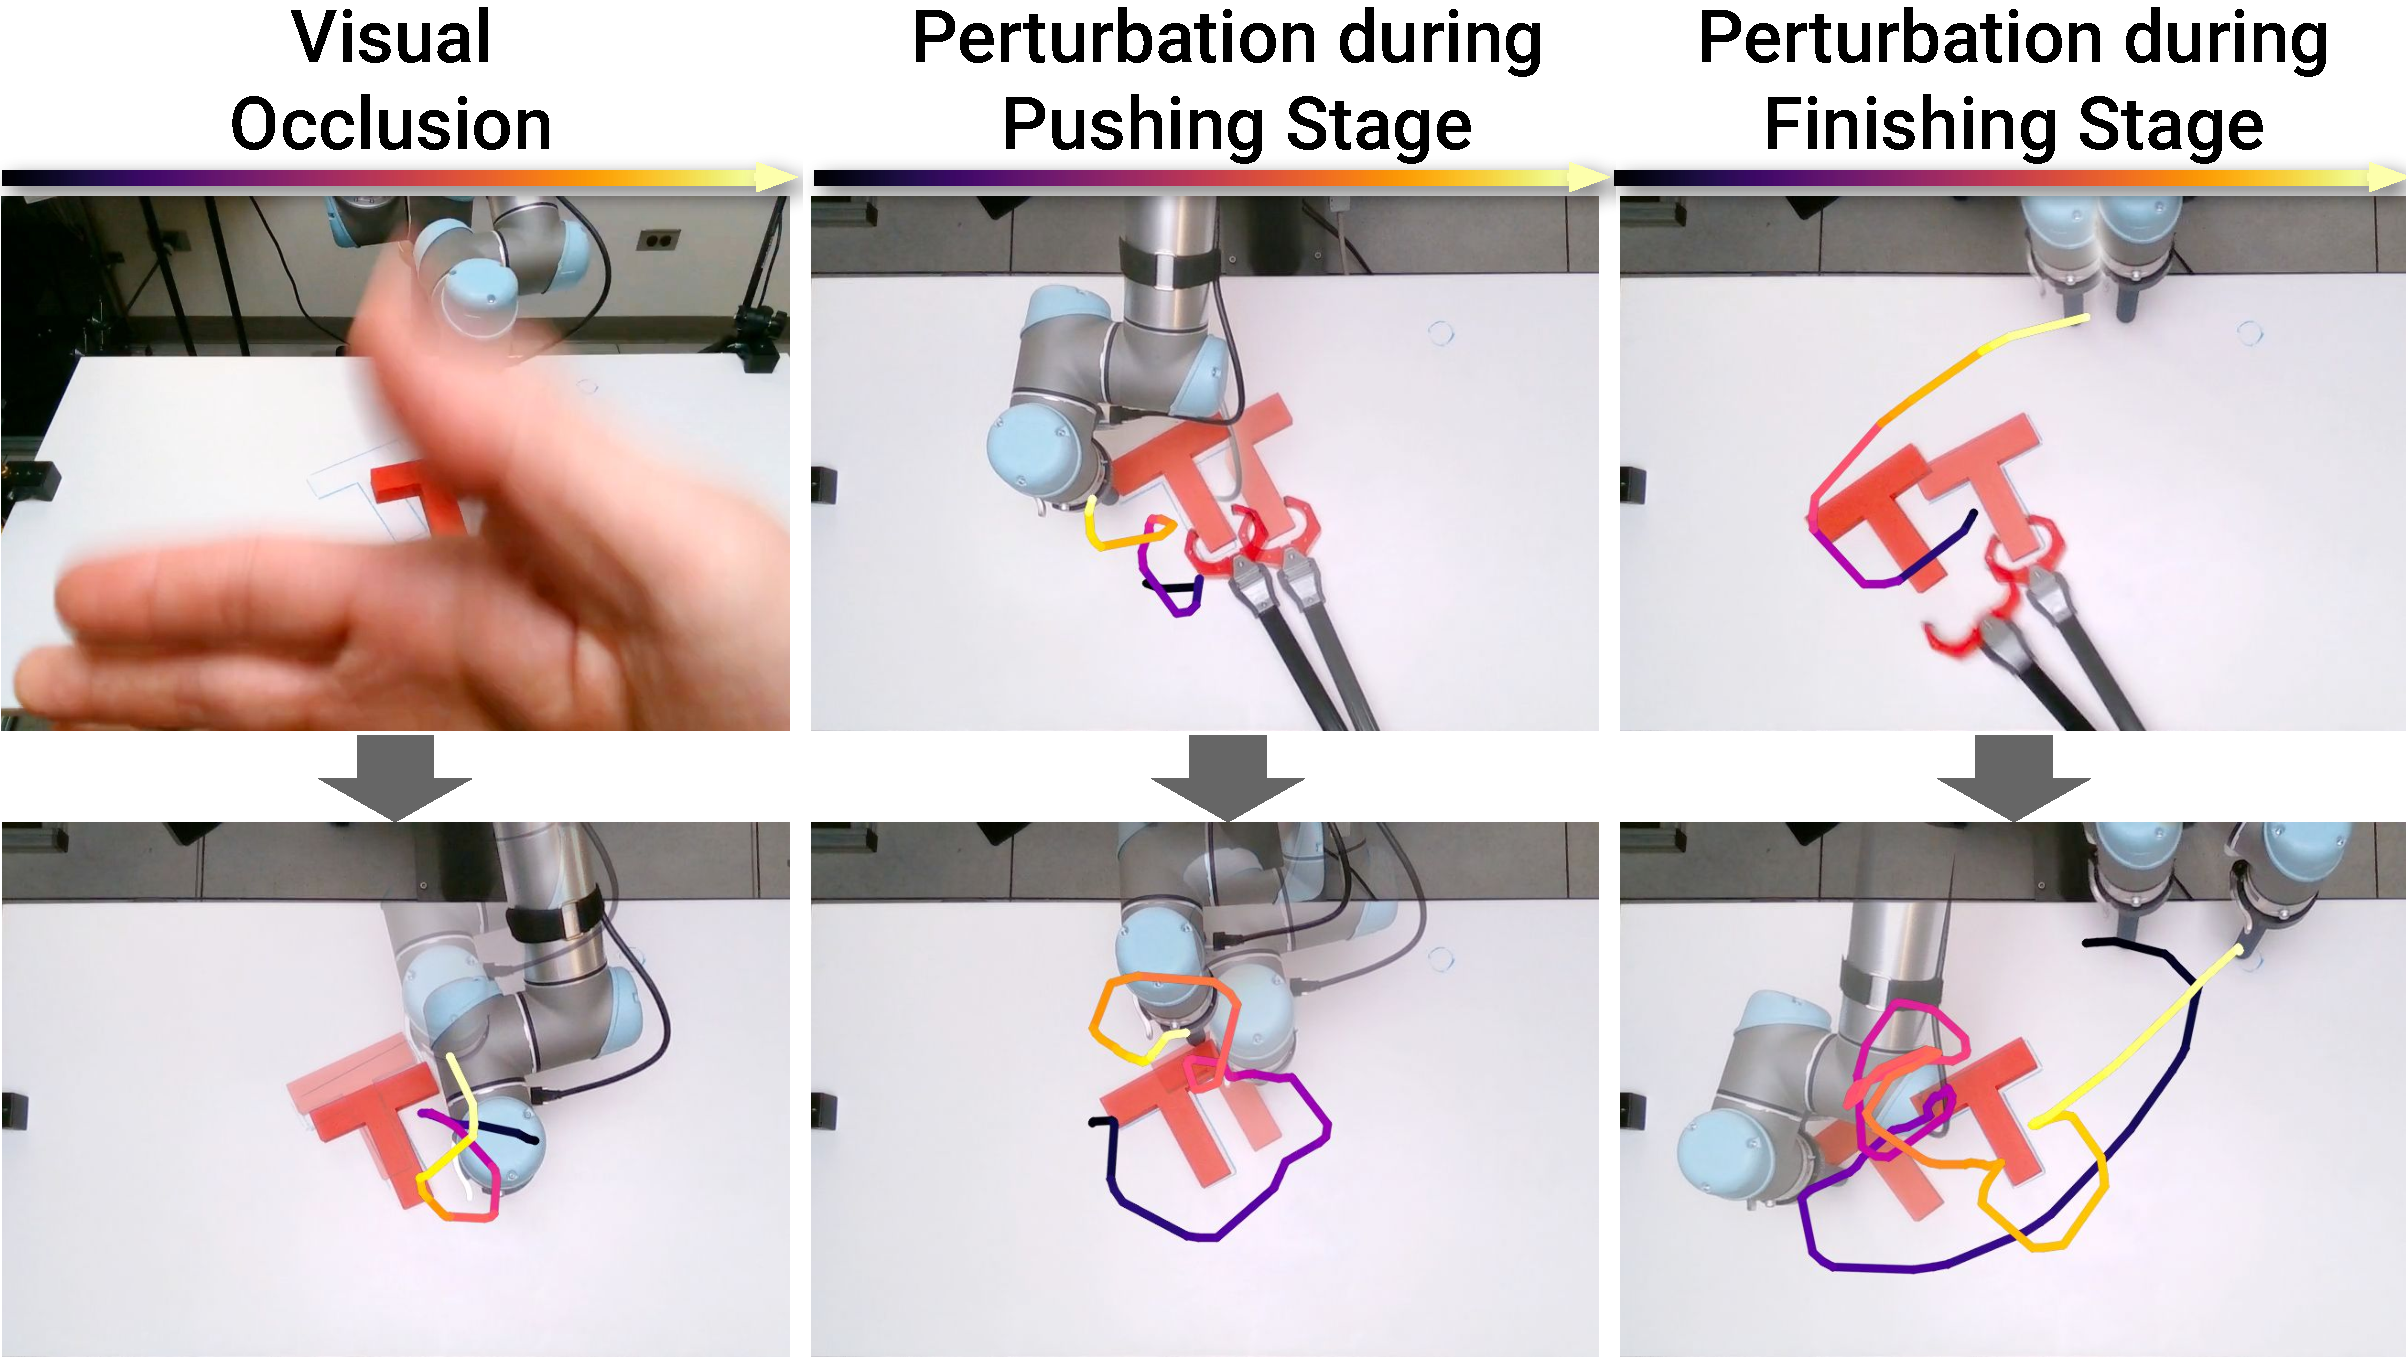
\includegraphics[width=\linewidth]{figure/real_robustness.pdf}

\caption{\textbf{Robustness Test for Diffusion Policy.}
\label{fig:robustness}
\textbf{Left}: A waving hand in front of the camera for 3 seconds causes slight jitter, but the predicted actions still function as expected.
\textbf{Middle}: Diffusion Policy immediately corrects shifted block position to the goal state during the pushing stage.
\textbf{Right}: Policy immediately aborts heading to the end zone, returning the block to goal state upon detecting block shift. This novel behavior was never demonstrated.
Please check the videos in the supplementary material. }

\vspace{-4mm}
\end{figure}

\textbf{Robustness against perturbation}
Diffusion Policy's robustness against visual and physical perturbations was evaluated in a separate episode from experiments in Tab \ref{tab:real_pusht}. As shown in Fig \ref{fig:robustness}, three types of perturbations are applied.
1) The front camera was blocked for 3 secs by a waving hand (left column), but the diffusion policy, despite exhibiting some jitter, remained on-course and pushed the T block into position.
2) We shifted the T block while Diffusion Policy was making fine adjustments to the T block's position. Diffusion policy immediately re-planned to push from the opposite direction, negating the impact of perturbation.
3) We moved the T block while the robot was en route to the end-zone after the first stage's completion. The Diffusion Policy immediately changed course to adjust the T block back to its target and then continued to the end-zone. This experiment indicates that Diffusion Policy may be able to \textbf{synthesize novel behavior} in response to unseen observations.

\begin{figure}[t]
\centering
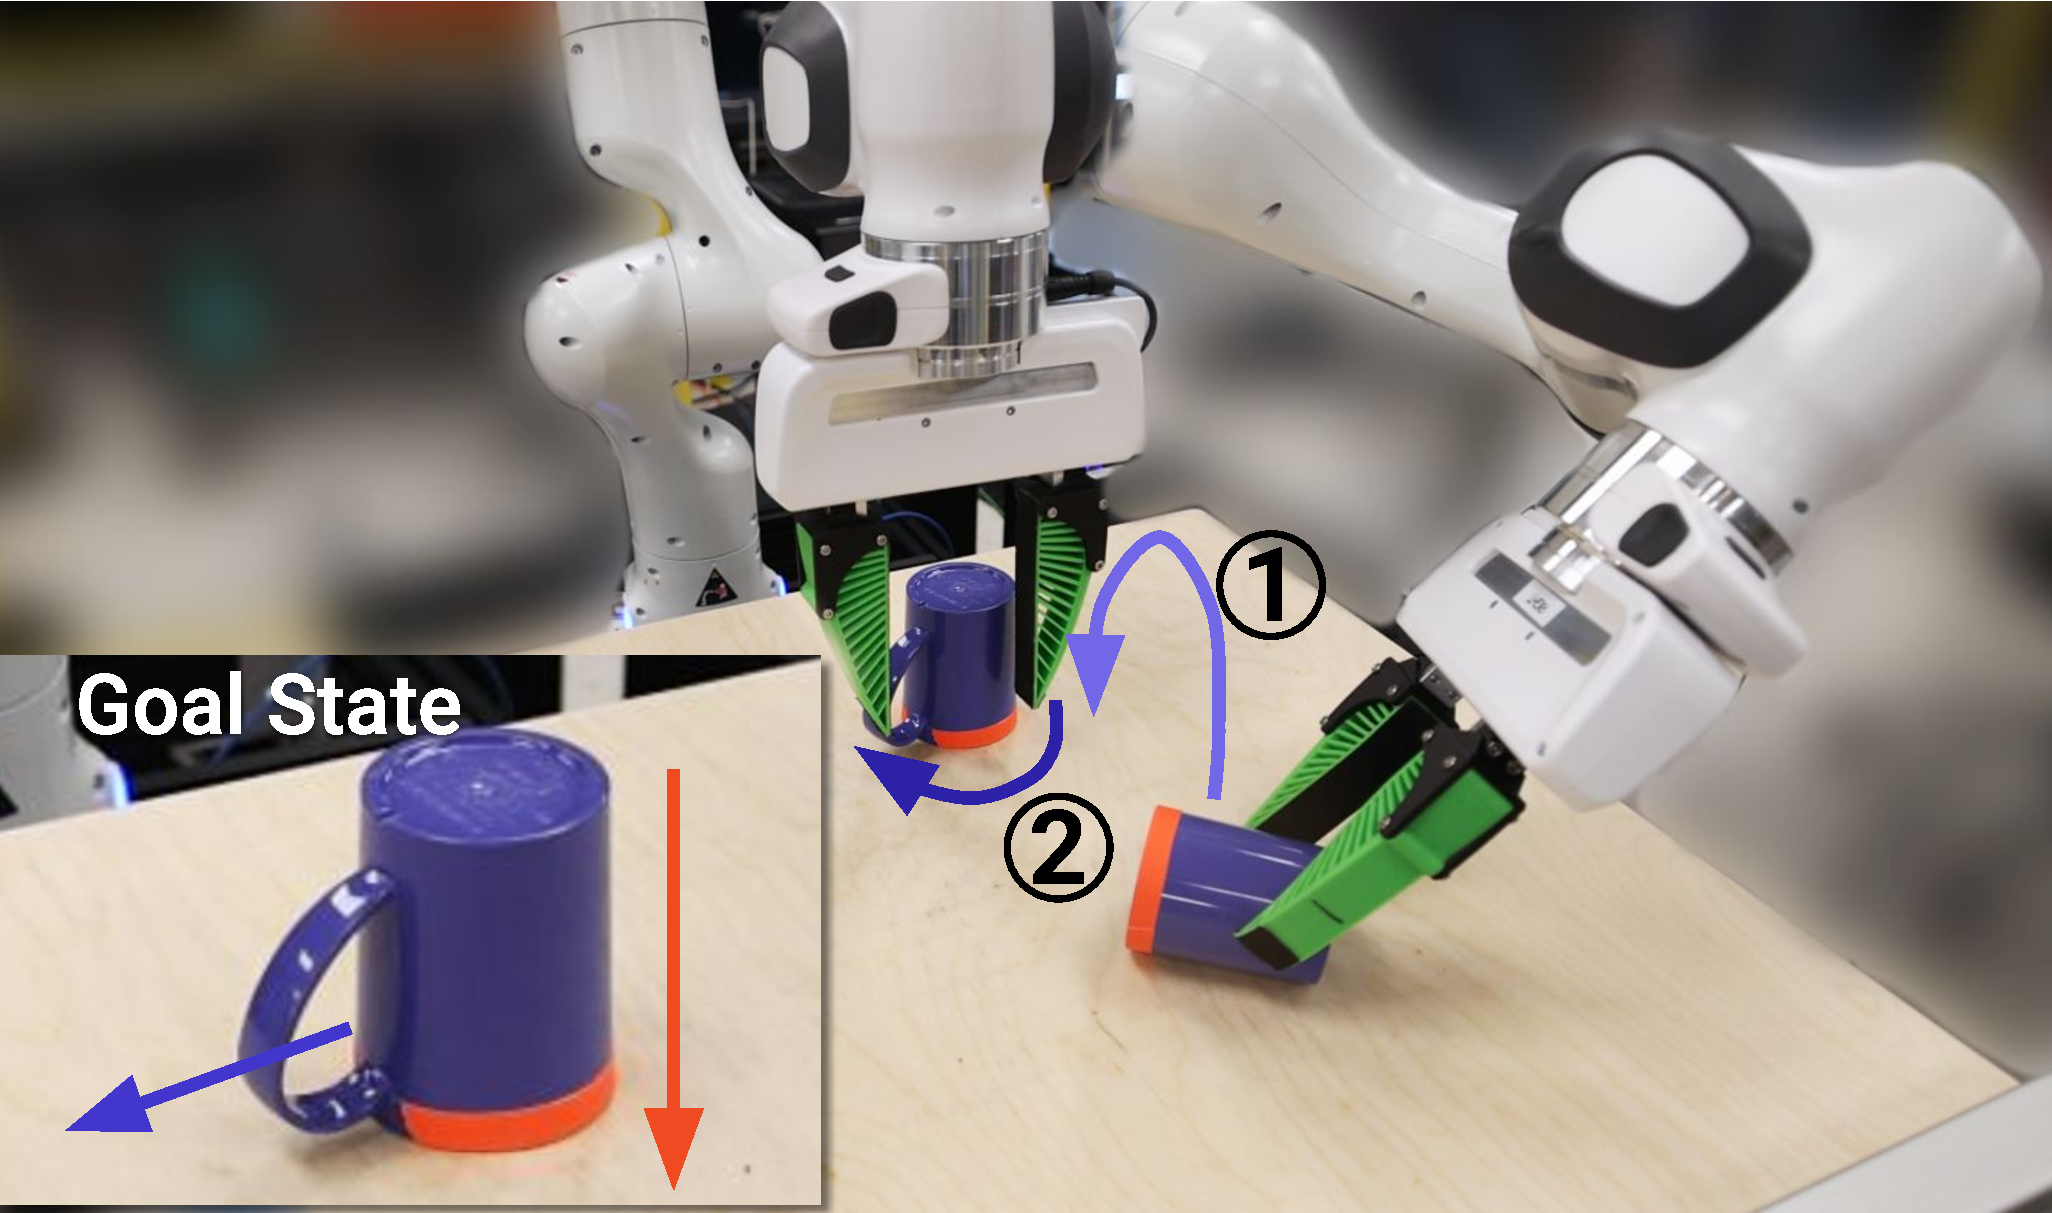
\includegraphics[width=0.9\linewidth]{figure/mug_task.pdf}

\vspace{1.5mm}
\begin{tabular}{c|c|c|c}
\toprule
        & Human & LSTM-GMM & Diffusion Policy \\
\midrule
Succ \% & 1.0   & 0.0      & 0.9             \\
\bottomrule
\end{tabular}

\caption{
\textbf{6DoF Mug Flipping Task.}
\label{fig:mug_task}
The robot needs to
\textcircled{\raisebox{-0.9pt}{1}} Pickup a randomly placed mug and place it lip down (marked orange).
\textcircled{\raisebox{-0.9pt}{2}} Rotate the mug such that its handle is pointing left.
}

\vspace{-4mm}
\end{figure}

\begin{figure}[t]
\centering
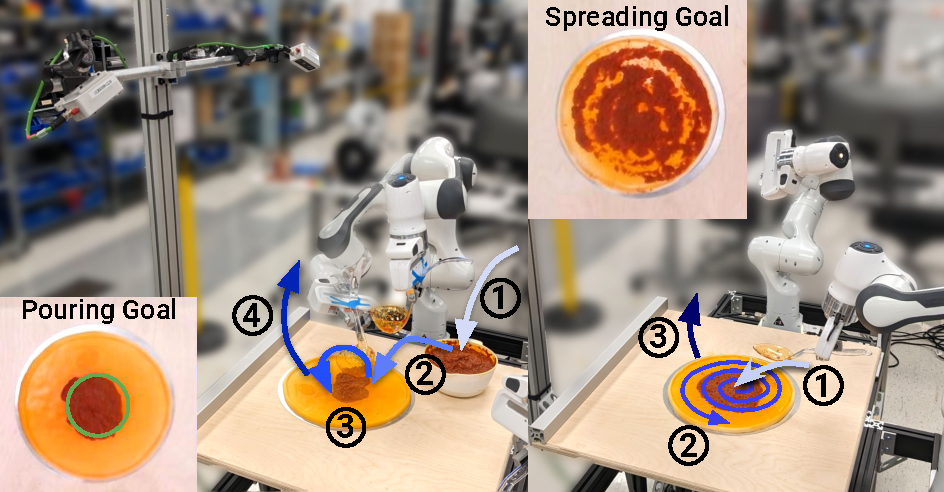
\includegraphics[width=\linewidth]{figure/real_sauce_setup.pdf}

\vspace{1.5mm}


\small
\begin{tabular}{r|c|c|c|c}
\toprule
         & \multicolumn{2}{c|}{Pour} & \multicolumn{2}{c}{Spread}    \\
         & IoU & Succ & Coverage & Succ \% \\
\midrule
Human  & 0.79 &     1.00  & 0.79  &    1.00      \\
\midrule
LSTM-GMM & 0.06 & 0.00  &  0.27  & 0.00           \\
Diffusion Policy  &  \textbf{0.74} &\textbf{0.79}   & \textbf{0.77}  & \textbf{1.00}   \\
\bottomrule
\end{tabular}



\caption{\textbf{Realworld Sauce Manipulation. }
\label{fig:real_sauce_manipulation}
[Left] \textbf{6DoF pouring Task.} The robot needs to \textcircled{\raisebox{-0.9pt}{1}} dip the ladle to scoop sauce from the bowl, \textcircled{\raisebox{-0.9pt}{2}} approach the center of the pizza dough, \textcircled{\raisebox{-0.9pt}{3}} pour sauce, and \textcircled{\raisebox{-0.9pt}{4}} lift the ladle to finish the task.
[Right] \textbf{Periodic spreading Task} The robot needs to \textcircled{\raisebox{-0.9pt}{1}} approach the center of the sauce with a grasped spoon, \textcircled{\raisebox{-0.9pt}{2}} spread the sauce to cover pizza in a spiral pattern, and \textcircled{\raisebox{-0.9pt}{3}} lift the spoon to finish the task.
}

\vspace{-4mm}
\end{figure}

\subsection{Mug Flipping Task}
The mug flipping task is designed to test Diffusion Policy's ability to handle complex \textbf{3D rotations} while operating close to the hardware's kinematic limits.
The goal is to reorient a randomly placed mug to have \textcircled{\raisebox{-0.9pt}{1}} the lip facing down \textcircled{\raisebox{-0.9pt}{2}} the handle pointing left, as shown in Fig. \ref{fig:mug_task}.
Depending on the mug's initial pose, the demonstrator might directly place the mug in desired orientation, or may use additional push of the handle to rotation the mug.
As a result, the demonstration dataset is highly multi-modal: grasp vs push, different types of grasps (forehand vs backhand) or local grasp adjustments (rotation around mug's principle axis), and are particularly challenging for baseline approaches to capture.

\textbf{Result Analysis.} Diffusion policy is able to complete this task with 90\% success rate over 20 trials. The richness of captured behaviors is best appreciated with the video. Although never demonstrated, the policy is also able to sequence multiple pushes for handle alignment or regrasps for dropped mug when necessary. For comparison, we also train a LSTM-GMM policy trained with a subset of the same data. For 20 in-distribution initial conditions, the LSTM-GMM policy never aligns properly with respect to the mug, and fails to grasp in all trials.

\subsection{Sauce Pouring and Spreading}
The sauce pouring and spreading tasks are designed to test Diffusion Policy's ability to work with \textbf{non-rigid} objects, \textbf{6 Dof} action spaces, and \textbf{periodic} actions in real-world setups. Our Franka Panda setup and tasks are shown in Fig \ref{fig:real_sauce_manipulation}. The goal for the \textbf{6DoF pouring task} is to pour one full ladle of sauce onto the center of the pizza dough, with performance measured by IoU between the poured sauce mask and a nominal circle at the center of the pizza dough (illustrated by the green circle in Fig \ref{fig:real_sauce_manipulation}).
The goal for the \textbf{periodic spreading task} is to spread sauce on pizza dough, with performance measured by sauce coverage.
Variations across evaluation episodes come from random locations for the dough and the sauce bowl.
The success rate is computed by thresholding with minimum human performance.
Results are best viewed in supplemental videos.
Both tasks were trained with the same Push-T hyperparameters, and successful policies were achieved on the first attempt.

The sauce pouring task requires the robot to remain stationary for a period of time to fill the ladle with viscous tomato sauce. The resulting idle actions are known to be challenging for behavior cloning algorithms and therefore are often avoided or filtered out. Fine adjustments during pouring are necessary during sauce pouring to ensure coverage and to achieve the desired shape.

The demonstrated sauce-spreading strategy is inspired by the human chef technique, which requires both a long-horizon cyclic pattern to maximize coverage and short-horizon feedback for even distribution (since the tomato sauce used often drips out in lumps with unpredictable sizes). Periodic motions are known to be difficult to learn and therefore are often addressed by specialized action representations \cite{yang2022periodic}.
Both tasks require the policy to self-terminate by lifting the ladle/spoon.




\textbf{Result Analysis.}
Diffusion policy achieves close-to-human performance on both tasks, with coverage 0.74 vs 0.79 on pouring and 0.77 vs 0.79 on spreading.
Diffusion policy reacted gracefully to external perturbations such as moving the pizza dough by hand during pouring and spreading.
Results are best appreciated with videos in the supplemental material.

LSTM-GMM performs poorly on both sauce pouring and spreading tasks. It failed to lift the ladle after successfully scooping sauce in 15 out of 20 of the pouring trials. When the ladle was successfully lifted, the sauce was poured off-centered. LSTM-GMM failed to self-terminate in all trials. We suspect LSTM-GMM's hidden state failed to capture sufficiently long history to distinguish between the ladle dipping and the lifting phases of the task. For sauce spreading, LSTM-GMM always lifts the spoon right after the start, and failed to make contact with the sauce in all 20 experiments.
